\documentclass[12pt]{report}
\usepackage[T1]{fontenc}
\usepackage[utf8]{inputenc}
\usepackage{libertinus}
\usepackage[italian]{babel}
\usepackage[most]{tcolorbox}
\usepackage{amsmath}
\usepackage{amsthm}
\usepackage{mathtools}
\usepackage{tabularx}
\usepackage{amssymb}
\usepackage{enumitem}
\usepackage{amsfonts}
\usepackage{centernot}
\usepackage{relsize}
\usepackage{mathrsfs}
\usepackage{bm}
\usepackage{xfrac}
\usepackage{lipsum}
\usepackage{bbm}
\usepackage{tikz}
\usepackage{cancel}
\usepackage{enumitem}
\usepackage{mathtools}
\usepackage{multicol}
\usepackage{float}
\usepackage{hyperref}
\usepackage{makecell}
\usepackage{listings}
\usepackage{xcolor}
\usepackage{pgfplots}
\usepackage{calligra}
\usepackage{subdepth}
\usepackage{tikz}
\usepackage{yhmath}
\usepackage{accents}
\usepackage{nicefrac}
\usetikzlibrary{angles, quotes, patterns}
\usepackage{circledsteps}
\date{}
\author{Alessandro Carella}
\title{Calcolabilità e complessità}
\setcounter{chapter}{0}
\setlist[enumerate]{label*=\arabic*.}
\setlength{\parindent}{0pt}
\definecolor{brickred}{RGB}{182, 50, 28}
\definecolor{darkred}{RGB}{139, 0, 0}
\definecolor{codegreen}{rgb}{0,0.6,0}
\definecolor{codegray}{rgb}{0.5,0.5,0.5}
\definecolor{codepurple}{rgb}{0.58,0,0.82}
\definecolor{backcolour}{rgb}{0.95,0.95,0.92}
\definecolor{darkblue}{rgb}{0,0,0.6}
\hypersetup{
	colorlinks=true,
	linkcolor=darkred,
	filecolor=darkred,
	urlcolor=darkred
}

\newcounter{theorem}
\newcounter{lemma}
\newcounter{corollary}
\newcounter{definition}
\newcounter{exercise}

\labelformat{theorem}{teorema #1}
\labelformat{lemma}{lemma #1}
\labelformat{corollary}{corollario #1}
\labelformat{definition}{definizione #1}
\labelformat{note}{nota #1}
\labelformat{example}{esempio #1}
\labelformat{exercise}{esercizio #1}

\newtcbtheorem[number within=chapter,use counter=lemma]{lemma}%
{Lemma}{arc=1mm,outer arc=1mm,colframe=cyan!55!black,fonttitle=\scshape,lefttitle=1mm,separator sign dash,description font=\bfseries,description delimiters={\flqq}{\frqq}}{lem}

\newtcbtheorem[no counter]
{note}{Nota}{blanker,breakable,left=5mm,before skip=10pt,after skip=10pt,borderline west={2.5mm}{0pt}{red!55},coltitle=black,fonttitle=\bfseries}{note}

\newtcbtheorem[no counter]
{example}{Esempio}{blanker,breakable,left=5mm,before skip=10pt,after skip=10pt,borderline west={2.5mm}{0pt}{yellow!55},coltitle=black,fonttitle=\bfseries}{exa}

\newtcbtheorem[number within=section,use counter=exercise]
{exercise}{Esercizio}{blanker,breakable,left=5mm,before skip=10pt,after skip=10pt,borderline west={2.5mm}{0pt}{yellow!55},coltitle=black,fonttitle=\bfseries}{exe}

\newtcbtheorem[no counter]
{assignment}{Traccia}{blanker,breakable,left=5mm,before skip=10pt,after skip=10pt,borderline west={2.5mm}{0pt}{brickred!65},coltitle=black,fonttitle=\bfseries}{asg}

\newtcbtheorem[number within=chapter,use counter=corollary]{corollary}%
{Corollario}{blanker,breakable,left=5mm,before skip=10pt,after skip=10pt,borderline west={2.5mm}{0pt}{cyan!55!black},coltitle=black,fonttitle=\bfseries}{cor}

\newtcbtheorem[number within=chapter,use counter=definition]{definition}%
{Definizione}{blanker,breakable,left=5mm,before skip=10pt,after skip=10pt,
	borderline west={2.5mm}{0pt}{green!55!black},coltitle=black,
	fonttitle=\scshape\bfseries,separator sign={:\hspace{0.5em}}}{def}

\newtcbtheorem[number within=chapter,use counter=theorem]{theorem}%
{Teorema}{blanker,breakable,left=5mm,before skip=10pt,after skip=10pt,borderline west={2.5mm}{0pt}{cyan!55!black},coltitle=black,fonttitle=\bfseries, separator sign={:\hspace{0.5em}}}{th}

\tcolorboxenvironment{proof}{blanker,breakable,left=5mm,before skip=10pt,after skip=10pt,borderline west={2.5mm}{0pt}{cyan!55!black}}
\newcommand{\namerefl}[1]{%
	\bgroup
	\let\nmu\MakeLowercase
	\nameref{#1}\egroup}

\newcommand{\nmu}{}
\newcommand{\wbar}[1]{%
	\accentset{\mbox{\rule{0.55em}{0.5pt}}}{#1}%
}

\lstdefinestyle{pascalstyle}{
	backgroundcolor=\color{backcolour},   
	commentstyle=\color{codegreen},
	keywordstyle=\color{blue}\bfseries,
	numberstyle=\tiny\color{codegray},
	stringstyle=\color{codepurple},
	basicstyle=\ttfamily\footnotesize,
	breakatwhitespace=false,         
	breaklines=true,                 
	captionpos=b,                    
	keepspaces=true,                 
	numbers=left,                    
	numbersep=5pt,                  
	showspaces=false,                
	showstringspaces=false,
	showtabs=false,                  
	tabsize=2,
	language=Pascal
}

\lstdefinestyle{normalstyle}{
	backgroundcolor=\color{backcolour},   
	commentstyle=\color{codegreen},
	keywordstyle=\color{blue}\bfseries,
	numberstyle=\tiny\color{codegray},
	stringstyle=\color{codepurple},
	basicstyle=\ttfamily\footnotesize,
	breakatwhitespace=false,         
	breaklines=true,                 
	captionpos=b,                    
	keepspaces=true,                 
	numbers=left,                    
	numbersep=5pt,                  
	showspaces=false,                
	showstringspaces=false,
	showtabs=false,                  
	tabsize=2,
}

\begin{document}
	{
		\let\cleardoublepage\clearpage
		\maketitle
		\tableofcontents
	}
	\chapter{Automi e linguaggi}
	\section{Automi finiti}
	Gli automi finiti sono un buon modello per computer una quantità estremamente di memoria che permette di fare molte cose utili. Il sistema di controllo per una porta automatica è un esempio di tale dispositivo. \\
	Gli automi finiti e la loro controparte probabilistica, le \textit{catene di Markov} sono utili strumenti quando cerchiamo di riconescere pattern in dati. Questi dispositivi sono usati nell'elaborazione vocale e nel riconoscimento ottico dei caratteri. Le catene di Markov sono state perfino usate per modellare e predire i cambiamenti dei prezzi nei mercati finanzieri.
	\paragraph{Definizione formale di automa finito} \quad \\
	\begin{definition}{\nmu Automa finito}{automa_finito}
		Un \textit{automa finito} è una quintupla $(Q, \sum, \delta, q_0, F)$ dove:
		\begin{enumerate}
			\item $Q$ è un insieme finito chiamato l'insieme degli \textit{stati};
			\item $\sum$ è un insieme finito chiamato \textit{alfabeto};
			\item $\delta: Q \times \sum \to Q$ è la \textit{funzione di transizione};
			\item $q_0 \in Q$ è lo \textit{stato iniziale};
			\item $F \subseteq Q$ è l'\textit{insieme degli stati accettanti.}
		\end{enumerate}
	\end{definition}
	Consideriamo il seguente automa $M_1$:
	\begin{figure}[H]
		\centering
		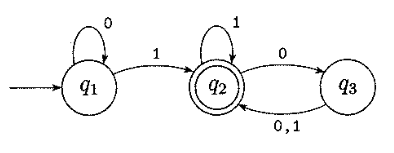
\includegraphics[width=.7\textwidth]{images/automa_finito_def}
	\end{figure}
	Possiamo descrivere $M_1$ formalmente ponendo $M_1 = (Q, \sum, \delta, q_1, F)$ ove:
	\begin{enumerate}
		\item $Q = \{q_1, q_2, q_3\}$;
		\item $\sum = \{0, 1\}$;
		\item $\delta$ è descritta come segue:
		\begin{center}
			\begin{tabular}{c|cc}
				& 0     & 1     \\ \hline
				$q_1$ & $q_1$ & $q_2$ \\
				$q_2$ & $q_3$ & $q_2$ \\
				$q_3$ & $q_2$ & $q_2$
			\end{tabular}
		\end{center}
		\item $q_1$ è lo stato iniziale;
		\item $F = \{q_2\}$
	\end{enumerate}
	Se $A$ è l'insieme di tutte le stringhe che la macchina $M$ accetta, diciamo che $A$ è il \textit{linguaggio della macchina M} e scriviamo $L(M) = A$. Diciamo che \textit{M riconosce A} o che \textit{M accetta A}. Poichè il termine \textit{accetta} ha significati diversi quando ci riferiamo a macchine che accettano stringhe e macchine che accettano linguaggi, per evitare confusione preferfiamo per i linguaggi il termine \textit{riconosce}. \\
	Una macchina può accettare diverse stringhe, ma riconosce sempre soltanto un linguaggio. Se la macchina non accetta alcuna stringa, essa riconosce ancora un lingauggio, il linguaggio vuoto $\emptyset$. \\
	Nel nostro esempio, sia:
	\[
	A = \{w \mid w \text{ contiene almeno un 1 e un numero pari di 0 segue l'ultimo 1}\}
	\] 
	\paragraph{Definizione formale di computazione} \quad \\
	Finora abbiamo descritto gli automi finiti informalmente, usando diagrammi di stato, e con una definizione formale, come una quintupla. La descrizione informale è più facile da comprendere all'inizio, ma la definizione formale è più utile per rendere la notazione precisa, risolvendo ogni ambiguità. \\
	Facciamo lo stesso per la computazione di un automa finito. \\
	Sia $M = (Q, \sum, \delta, q_0, F)$ un automa finito e sia $w = w_1w_2\cdots w_n$ una stringa dove ogni $w_i$ è un elemento dell'alfabeto $\sum$. Allora $M$ \textit{accetta w} se esiste una sequenza di stati $r_0, r_1, \dots, r_n$ in $Q$ con tre condizioni:
	\begin{enumerate}
		\item $r_0 = q_0$;
		\item $\delta(r_i, w_{i+1}) = r_{i+1}$ per $i = 0, \dots, n - 1$;
		\item $r_n \in F$.
	\end{enumerate} 
	La prima condizione afferma che la macchina inizia nello stato inziale. La seconda condizione afferma che la macchina passa da stato a stato in base alla funzione di transizione. La terza condizione afferma che la macchina accetta il suo input se termina la lettura in uno stato accettante. Diciamo che $M$ \textit{riconosce il linguaggio A} se $A = \{w \mid M \text{ accetta } w\}$.
	\begin{definition}{\nmu Linguaggio regolare}{linguaggio_regolare}
		Un linguaggio è chiamato un \textit{linguaggio regolare} se un automa finito lo riconosce. 
	\end{definition}
	\paragraph{Le operazioni regolari} \quad \\
	Dopo aver introdotto e definito gli automi finiti e i linguaggi regolari, iniziamo a studiarne le proprietà. In aritmetica, gli oggetti di base sono i numeri e gli strumenti sono le operazioni per trattarli, come $+$ e $\times$. Nella teoria della computazione, gli oggetti sono i linguaggi e gli strumenti includono operzioni specificatamente progettate per trattarli. Definiamo tre operazioni sui linguaggi, chiamate \textit{operazioni regolari}, e le usiamo per studiare le proprietà dei linguaggi regolari. 
	\begin{definition}{\nmu Operazioni regolari}{operazioni_regolari}
		Siano $A$ e $B$ linguaggi. Definiamo le operazioni regolari \textit{unione, concatenazione} e \textit{star} come segue:
		\begin{itemize}
			\item \textbf{Unione:} $A \cup B = \{x \mid x \in A \text{ o } x \in B\}$
			\item \textbf{Concatenazione:} $A \circ B = \{xy \mid x \in A \text{ e } y \in B\}$
			\item \textbf{Star}: $A^* = \{x1x2\dots x_k \mid k \geq 0 \text{ e ogni } x_i \in A\}$
		\end{itemize}
	\end{definition} 
	\begin{example}{}{}
		Sia $\sum$ l'alfabeto standard a 26 lettere $\{a, b, \dots, z\}$. Se $A = \{good,\ bad\}$ e $B = \{boy,\ girl\}$, allora:
		\begin{align*}
			A \cup B &= \{\text{good, bad, boy, girl}\} \\
			A \circ B &= \{\text{goodboy, goodgirl, badboy, badgirl}\} \\
			A^* &= \{\epsilon, \text{good, bad, goodgood, goodbad, badgood, badbad, goodgoodgood, goodgoodbad, \dots }\}
		\end{align*}
	\end{example}
	Sia $\mathbbm{N} = \{1, 2, 3, \dots\}$ l'insieme dei numeri naturali. Quando diciamo che $\mathbbm{N}$ è \textit{chiuso rispetto alla moltiplicazione}, intediamo che per ogni $x$ e per ogni $y$ in $\mathbbm{N}$, il prodotto $x \times y \in \mathbbm{N}$. Invece $\mathbbm{N}$ non è chiuso rispetto alla divisione, poichè $1$ e $2$ sono in $\mathbbm{M}$ ma $\sfrac{1}{2} \notin \mathbbm{N}$.  \\
	In generale, una classe di oggetti è \textit{chiusa} rispetto a un'operazione se l'applicazione di questa operazioni a elementi della classe restituisce un oggetto ancora nella classe. Mostriamo che la classe dei linguaggi regolari è chiusa rispetto a tutte e tre le operazioni regolari. 
	\begin{theorem}{\nmu Chiusura unione}{unione_chiusura}
		La classe dei linguaggi regolari è chiusa rispetto all'operazioni di unione. \\
		In altre parole, se $A_1$ e $A_2$ sono linguaggi regolari, lo è anche $A_1 \cup A_2$. 
	\end{theorem} 
	Quindi, abbiamo due linguaggi regolari, $A_1$ e $A_2$, e vogliamo mostrare che anche $A_1 \cup A_2$ è regolare. Poichè $A_1$ e $A_2$ sono regolari, sappiamo che sono riconosciuti da degli automi finiti. Quindi per provare che $A_1 \cup A_2$ è regolare, dobbiamo esibire un automa finito, $M$, che riconosce $A_1 \cup A_2$. 
	\begin{proof}
		Supponiamo che $M_1$ riconosca $A_1$, dove $M_1 = (Q_1, \sum, \delta_1, q_1, F_1)$ ed $M_2$ riconosca $A_2$, dove $M_2 = (Q_2, \sum, \delta_2, q_2, F_2)$. \\
		Costruiamo $M$ che riconosce $A_1 \cup A_2$ dove $M = (Q, \sum, \delta, q_0, F)$.
		\begin{enumerate}
			\item $Q = \{(r_1, r_2) \mid r_1 \in Q_1 \text{ e } r_2 \in Q_2\}$. \\
			Questo insieme è il \textit{prodotto cartesiano} degli insiemi $Q_1$ e $Q_2$ ed è denotato con $Q_1 \times Q_2$.
			\item $\sum$, l'alfabeto è lo stesso di $M_1$ e $M_2$. In questo teorema e in quelli successivi, assumiamo per semplicità che sia $M_1$ che $M_2$ abbiamo stesso alfabeto di simboli. Tuttavia, se così non fosse, $\sum = \sum_1 \cup \sum_2$.
			\item $\delta$, la funzione di transizione, è definita come segue. Per ogni $(r_1, r_2) \in Q$ e ogni $a \in \sum$, sia
			\[
			\delta((r_1, r_2), a) = (\delta_1(r_1, a), \delta_2(r_2, a))
			\]
			\item $q_0$ è la coppia $(q_1, q_2)$.
			\item $F$ è l'insieme delle coppie in cui l'uno o l'altro elemento è uno stato accettante di $M_1$ o $M_2$. Possiamo scriverlo come
			\[
			F = \{(r_1, r_2) \mid r_1 \in F_1 \text{ o } r_2 \in F_2\}
			\]
			Questa espressione è uguale a $F=(F_1 \times Q_2) \cup (Q_1 \times F_2)$
		\end{enumerate}
	\end{proof}  
	Abbiamo mostrato che l'unione di due linguaggi regolari è regolare, provanto che la classe dei linguaggi regolari è chiusa rispetto all'operazione di unione. Ora mostriamo che la classe dei linguaggi regolari è chiusa rispetto all'operazione di concatenazione. 
	\begin{theorem}{\nmu Chiusura concatenazione}{chiusura_contenazione}
		La classe dei linguaggi regolari è chiusa rispetto all'operazione di concatenazione. \\
		In altre parole, se $A_1$ e $A_2$ sono linguaggi regolari, allora lo è anche $A_1 \circ A_2$.
	\end{theorem}
	Per provare questo teorema, possiamo iniziare con gli automi finiti $M_1$ ed $M_2$ che riconoscono i linguaggi regolari $A_1$ ed $A_2$. Ma ora, invece di costruire $M$ che accetta l'input se $M_1$ o $M_2$ lo accetta, esso deve accettare se il suo input può essere diviso in due parti, tali che $M_1$ accetta la prima parte ed $M_2$ accetta la seconda parte. Il problema è che $M$ non sa dividere il suo input. Per risolvere questo problema, introduciamo una tecnica chiamata \textit{non determinismo}. 
	\section{Non determinismo}
	Negli esempi visti precedentemente, ogni passo di una computazione seguiva univocamente dal passo precedente. Quando la macchina è in un dato stato e legge il simbolo di input successivo, sappiamo qual è lo stato successivo, esso è univocamente determinato. In questo caso parliamo di computazione \textit{deterministica}. In una macchina \textit{non deterministica}, possono esistere diverse scelta per lo stato successivo in ogni punto. \\
	Il non determinismo è una generalizzazione del determinismo, quindi ogni automa finito deterministico è automaticamente un automa finito non deterministico. \\
	Consideriamo il seguente automa:
	\begin{figure}[H]
		\centering
		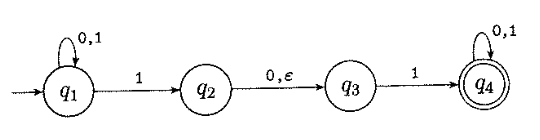
\includegraphics[width=0.7\textwidth]{images/automa_non_deterministico}
	\end{figure}
	La differenza tra un automa finito deterministico, DFA, e un automa finito non deterministico, indicato con NFA, è evidente. In primo luogo, ogni stato di un DFA ha sempre esattamente un arco usente per ogni simbolo nell'alfabeto. L'NFA viola questa regola, infatti, lo stato $q_1$ dell'automa della figura precedente, ha un arco uscente per 0, ma ne ha due per 1. In un NFA, uno stato può avere zero, uno, o più archi uscenti per ogni simbolo dell'alfabeto. \\
	Inoltre, in un DFA, le etichette sugli archi di transizione sono simboli dell'alfabeto. Questo NFA ha un arco con etichetta $\epsilon$. \\
	Durante la computazione di un NFA, quando si giunge ad uno stato con più modi per procedere, la macchina si divide in più copie di sè stessa e segue tutte le possibilità in parallelo. Infine, se una qualunque di queste copie della macchina è in uno stato accettante alla fine dell'input, l'NFA accetta la stringa di input. \\
	Il non determinismo può essere visto come una specie di computazione parallela dove ``processi'' multipli indipendenti o ``threads'' possono essere eseguiti contemporaneamente. Un altro modo per considerare una computazione non deterministica è vederla come un albero di possibilità. La radice dell'albera corrisponde all'inizio della computazione. Considerando sempre l'automa precedente, l'albero di computazione è il seguente:
	\begin{figure}[H]
		\centering
		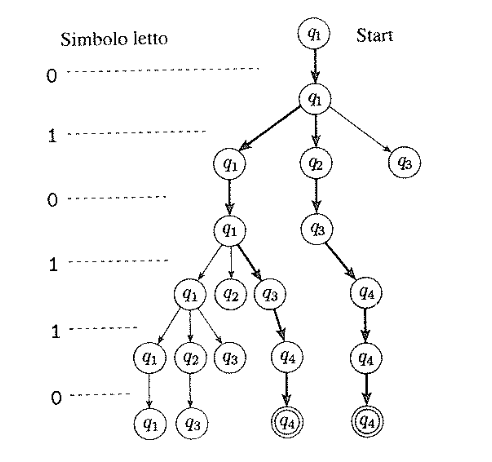
\includegraphics[width=1.0\textwidth]{images/albero_computazione}
		\caption{La computazione dell'automa precedente su 010110}
	\end{figure}
	\paragraph{Definizione formale di automa finito non deterministico} \quad \\
	La definizione formale di automa finito non deterministico è simile a quella di automa finito deterministico. Essi differiscono nel tipo di funzione di transizione. In un DFA, la funzione di transizione prende uno stato e un simbolo di input e produce lo stato successivo. In un NFA, la funzione di transizione prende uno stato e un simbolo di input o \textit{la stringa vuota} e produce l'\textit{insieme dei possibili stati successivi}. 
	\begin{definition}{\nmu Automa finito non deterministico}{automa_non_deterministico}
		Un \textit{automa finito non deterministico} è una quintupla $(Q, \sum, \delta, q_0, F)$ dove
		\begin{enumerate}
			\item $Q$ è un insieme finito di stati,
			\item $\sum$ è un alfabeto finito,
			\item $\delta: Q \times \sum_\epsilon \to \mathscr{P}(Q)$ è la funzione di transizione,
			\item $q_0 \in Q$ è lo stato iniziale,
			\item $F \subseteq Q$ è l'insieme degli stati di accettazione.
		\end{enumerate}
	\end{definition}
	\begin{example}{}{}
		Riconsideriamo il seguente NFA $N_1$:
		\begin{figure}[H]
			\centering
			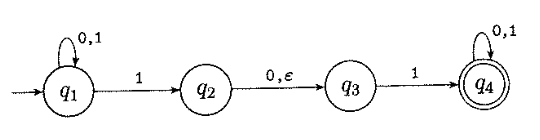
\includegraphics[width=.7\textwidth]{images/automa_non_deterministico}
		\end{figure}
		La descrizione formale di $N_1$ è $(Q, \sum, \delta, q_1, F)$ dove
		\begin{enumerate}
			\item $Q = \{q_1, q_2, q_3, q_4\}$
			\item $\sum = \{0, 1\}$
			\item $\delta$ è data da
			\begin{center}
				\begin{tabular}{c|ccc}
					& 0          & 1                 & $\epsilon$  \\ \hline
					$q_1$ & $\{q_1\}$  & $\{q_1, q_2\}$    & $\emptyset$ \\
					$q_2$ & $\{q_3\}$  & $\emptyset$       & $\{q_3\}$   \\
					$q_3$ & $\emptyset$ & $\{q_4\}$         & $\emptyset$ \\
					$q_4$ & $\{q_4\}$  & $\{q_4\}$         & $\emptyset$
				\end{tabular}
			\end{center}
			\item $q_1$ è lo stato inziale
			\item $F = \{q_4\}$
		\end{enumerate}
	\end{example}
	La definzione formale di computazione per un NFA è simile a quella per un DFA. Sia $N=(Q, \sum, \delta, q_0, F)$ un NFA e sia $w$ una stringa sull'alfabeto $\sum$. Diciamo che $N$ \textit{accetta} $w$ se possiamo scrivere $w$ come $w = y_1y_2\dots y_m$, dove ciascun $y_i$ è un elemento di $\sum_\epsilon$ ed esiste una sequenza di stati $r_0, r_1, \dots, r_n$ in $Q$ con tre condizioni:
	\begin{enumerate}
		\item $r_0 = q_0$
		\item $r_{i+1} \in \delta(r_i, y_{i+1})$ per $i = 0, \dots, m-1$
		\item $r_m \in F$
	\end{enumerate}
	\paragraph{Equivalenza tra gli NFA e i DFA} Gli automi finiti deterministici e quelli non deterministici riconoscono la stessa classe di linguaggi. Diciamo che due macchine sono \textit{equivalenti} se esse riconoscono lo stesso linguaggio. 
	\begin{theorem}{\nmu Equivalenza NFA e DFA}{equivalenza_automi}
		Per ogni automa finito non deterministico esiste un automa finito deterministico equivalente.
	\end{theorem}
	Se un linguaggio è riconosciuto da un NFA, allora dobbiamo mostrare l'esistenza di un DFA che lo riconosce. L'idea è trasformare l'NFA in un DFA equivalente che simula l'NFA. 
	\begin{proof} Sia $N = (Q, \sum, \delta, q_0, F)$ l'NFA che riconosce un linguaggio $A$. Costruiamo un DFA $M = (Q', \sum, \delta',q_0', F')$ che riconosce $A$. Prima di fare la costruzione completa, consideriamo inizialmente il caso più semplice in cui $N$ non ha $\epsilon-$archi.
		\begin{enumerate}
			\item $Q'=\mathscr{P}(Q)$ \\
			Ogni stato di $M$ è un insieme di stati di $N$. 
			\item Per $R \in Q'$ e $a\in\sum$, sia $\delta'(R, a) = \{q \in Q \mid q \in \delta(r, a)\}$ per qualche $r \in R$ \\
			Se $R$ è uno stato di $M$, esso è anche un insieme di stati di $N$. Qunado  $M$ legge un simbolo $a$ nello stato $R$. Poichè da ogni stato si può andare in un insieme di stati, prendiamo l'unione di tutti questi insiemi. Un altro modo per scrivere quest'espressione è:
			\[
			\delta'(R, a) = \bigcup_{r\in R}\delta(r, a)
			\]
			\item $q_0'= \{q_0\}$
			\item $F'=\{R \in Q' \mid R \text{ contiene uno stato accettante di } N\}$
		\end{enumerate}
	Ora dobbiamo considerare gli $\epsilon$-archi. Per farlo introduciamo qualche ulteriore notazione. Per ogni stato $R$ di $M$, definiamo $E(R)$ come la collezione di stati che possono essere raggiunti dagli elementi di $R$ proseguendo solo con $\epsilon$-archi, includendo gli stessi elementi di $R$. Formalmente, per $R \subseteq Q$ sia
	\[
	E(R) = \{q \mid q \text{ può essere raggiundo da } R \text{ attraverso 0 o più } \epsilon-archi\}
	\]
	Modifichiamo la funzione di transizione di $M$ ponendo le dita su tutti gli stati che possono essere raggiunti proseguendo attraverso $\epsilon$-archi dopo ogni passo. Sostituendo $\delta(r, a)$ con $E(\delta(r, a))$ realizziamo questo effetto.
	La funzione di transizione è la seguente.
	\[
	\delta'(R, a) = \{q \in Q \mid q \in E(\delta(r, a)) \text{ per qualche } r\in R\}
	\]
	Inoltre, dobbiamo modificare lo stato inziale di $M$ per muovere inizalmente le dita su tutti i possibili stati che possono essere raggiunti dallo stato iniziale di $N$ attraverso gli $\epsilon$-archi. Cambiare $q_0'$ in $E(\{q_0\})$ realizza questo risultato. Abbiamo così completato la costruzione del DFA $M$ che simula l'NFA $N$.
	\end{proof}
	\begin{corollary}{}{}
		Un linguaggio è regolare se e solo se qualche automa finito non deterministico lo riconosce.
	\end{corollary}
	Una direzione della condizione ``se e solo se'' afferma che unn linguaggio è regolare se qualche NFA lo riconosce. Tuttavia, abbiamo dismostrato che ogni NFA può essere trasformato in un DFA. Conseguentemente, se un NFA riconosce un linguaggio, lo fa anche qualche DFA, e quindi il linguaggio regolare. L'altra direzione della condizione ``se e solo se'' afferma che un linguaggio è regolare solo se qualche NFA lo riconosce. Questa condizione è vera perchè un linguaggio regolare ha un DFA che lo riconosce e un DFA è anche un NFA. 
	\paragraph{Chiusura rispetto alle operazioni regolari} \quad \\
	Torniamo alla chiusura della classe dei linguaggi regolari rispetto alle operazioni regolari. Dobbiamo provare che l'unione, la concatenazione e lo star di linguaggi regolari sono ancora regolari. 
	\begin{theorem}{}{}
		La classe dei linguaggi regolari è chiusa rispetto all'operazione di unione.
	\end{theorem}
	Abbiamo i linuaggi regolari $A_1$ ed $A_2$ e vogliamo provare che $A_1 \cup A_2$ è regolare. L'idea è provare che due NFA, $N_1$ ed $N_2$ per $A_1$ ed $A_2$, e comporli in un nuovo NFA, $N$. La macchina  $N$ deve accettare il suo input se $N_1$ o $N_2$ accetta questo input. La nuova macchina ha uno stato inziale che si dirama negli stati inziali delle vecchie macchine con $\epsilon$ archi.
	\begin{proof}
		Sia $N_1 = (Q_1, \sum, \delta_1, q_1, F)$ che riconosce $A_1$ ed $N_2 = (Q_2, \sum, \delta_2, q_2, F_2)$ che riconosce $A_2$. \\
		Costruiamo $N = (Q, \sum, \delta, q_0, F)$ per riconoscere $A_1\cup A_2$.
		\begin{enumerate}
			\item $Q = \{q_0\} \cup Q_1 \cup Q_2$ 
			\item Lo stato $q_0$ è lo stato inziale di \textit{N}
			\item L'insieme degli stati accettanti è $F = F_1 \cup F_2$
			\item Definiamo $\delta$ in modo che per ogni $q \in Q$ e $a \in \sum_\epsilon$
			\[
			\delta(q, a) = \begin{cases}
				\delta_1(q, a) & q\in Q_1 \\
				\delta_2(q, a) & q \in Q_2 \\
				\{q_1, q_2\} & q = q_0 \text{ e } a = \epsilon \\
				\emptyset & q = q_0 \text{ e } a \neq \epsilon
			\end{cases}
			\] 
		\end{enumerate}
	\end{proof}
	\begin{theorem}
		La classe dei linguaggi regolari è chiusa rispetto all'operazione di concantenazione.
	\end{theorem}
	L'idea è prendere due NFA, $N_1$ ed $N_2$, per $A_1$ ed $A_2$, e combinarli in un nuovo NFA $N$. Poniamo come stato inziale di $N$ lo stato inziale $N_1$. Gli stati accettanti di $N_1$ hanno degli ulteriori $\epsilon$-archi che non deterministicamente permettono di diramarsi in $N_2$ ogni volta che $N_1$ è in uno stato accettante, indicando che ha trovato un pezzo iniziale dell'input che costituisce una stringa in $A_1$. Gli stati accettandi di $N$ sono gli stati accettanti di $N_2$.
	\begin{proof}
		Sia $N_1 = (Q_1, \sum, \delta_1, q_1, F_1)$ che riconosce $A_1$ ed $N_2 = (Q_2, \sum, \delta_2, q_2, F_2)$ che riconosce $A_2$. \\
		Costruiamo $N = (Q, \sum,\delta, q_1, F_2)$ per riconoscere $A_1 \circ A_2$.
		\begin{enumerate}
			\item $Q = Q_1 \cup Q_2$
			\item Lo stato $q_1$ è uguale allo stato iniziale di $N_1$
			\item Gli stati accettanti $F_2$ sono uguale agli stati accettanti di $N_2$
			\item Definiamo $\delta$ in modo che per ogni $q \in Q$ e ogni $a \in \sum_\epsilon$
			\[
			\delta(q, a) = \begin{cases}
				\delta_1(q, a) & q \in Q_1 \text{ e } q \notin F_1 \\
				\delta_1(q, a) & q \in F_1 \text{ e } a \neq \epsilon \\
				\delta_1(q, a) \cup \{q_2\} & q \in F_1 \text{ e } a = \epsilon \\
				\delta_2(q, a) & q \in Q_2 
			\end{cases}
			\]
		\end{enumerate}
	\end{proof}
	\begin{theorem}{}{}
		La classe dei linguaggi regolari è chiusa rispetto all'operazione star.
	\end{theorem}
	Prendiamo un NFA $N_1$ per $A_1$ e lo modifichiamo per riconoscere $A_1^*$. L'NFA $N$ risultante accetterà il suo input quando esso può essere diviso in varie parti ed $N_1$ accetta ogni parte. Possiamo costruire $N$ come $N_1$ con $\epsilon$-archi supplementari che dagli stati accettanti ritornano allo stato iniziale. In questo modo, quando l'elaborazione giunge alla fine di una parte che $N_1$ accetta, la macchina $N$ ha la scelta di tornare indietro allo stato iniziale per provare a leggere un'altra parte che $N_1$ accetta. Inoltre, dobbiamo modificare $N$ in modo che accetti $\epsilon$, che è sempre un elemento di $A_1^*$.
	\begin{proof}
		Sia $N_1 = (Q_1, \sum, \delta_1, q_1, F_1)$ che riconosce $A_1$. \\
		Costruiamo $N = (Q, \sum, \delta, q_0, F)$ per riconoscere $A_1^*$.
		\begin{enumerate}
			\item $Q = \{q_0\} \cup Q_1$
			\item Lo stato $q_0$ è il nuovo stato iniziale. 
			\item $F = \{q_0\} \cup F_1$ 
			\item Definiamo $\delta$ in modo che per ogni $q \in Q$ e ogni $a \in \sum_\epsilon$
			\[
			\delta(q, a) = \begin{cases}
				\delta_1(q a) & q \in Q_1 \text{ e } q \notin F_1 \\
				\delta_1(q, a) & q \in F_1 \text{ e } a \neq \epsilon \\
				\delta_1(q, a) \cup \{q_1\} & q \in F_1 \text{ e } a = \epsilon \\
				\{q_1\} & q = q_0 \text{ e } a = \epsilon \\
				\emptyset & q = q_0 \text{ e } a \neq \epsilon
			\end{cases}
			\]
		\end{enumerate}
	\end{proof}
\end{document}
